\pdfoutput=1
\documentclass[11pt]{article}

\usepackage[margin=1in]{geometry}
\usepackage[T1]{fontenc}
\usepackage[utf8]{inputenc}
\usepackage{lmodern}
\usepackage{microtype}
\usepackage{amsmath,amssymb,mathtools}
\usepackage{booktabs}
\usepackage{graphicx}
\usepackage{caption}
\usepackage{subcaption}
\usepackage{enumitem}
\usepackage{array}
\usepackage{multirow}
\usepackage{natbib}
\usepackage[hidelinks]{hyperref}
\usepackage{xurl}
\usepackage{siunitx}
\usepackage{authblk}
\usepackage{float}

\graphicspath{{figures/}}
\setlist{nosep}
\setlength{\parskip}{0.35em}
\setlength{\parindent}{1em}
\sisetup{detect-all}

\title{Information Location under Matched Predictive Opportunity}
\author{Yukitake Miyamoto}
\affil{Independent Researcher, Japan}
\date{October 2026}

\begin{document}
\maketitle

\begin{abstract}
Model rankings are difficult to interpret when benchmark tasks differ both in how predictable the target is and in where the predictive signal is located. We construct a finite-support synthetic testbed with a known binary posterior and the same public semantic facts available to every learner. In three core conditions, an identical two-point posterior marginal is determined by either a current warning, dependency topology, or the order of earlier warnings; a fourth topology--history interaction condition matches Bayes Brier opportunity but not the full posterior marginal. Across 2,304 development runs of specified tabular, static-graph, size-control, and graph-plus-GRU systems, rankings are not uniform: the temporal system has better mean size-integrated normalized regret than the static system in both ordered-history conditions, while the topology and interaction contrasts reverse direction across opportunity levels. Large tabular--static gaps also appear in the current-state control, where topology and ordered history do not determine the posterior, so rankings cannot be read as direct measures of structural-information use. Exact expected-risk evaluation removes sampled evaluation-label noise. In selected post-hoc replays, learned content pathways lose prediction-relevant distinctions although the underlying input information remains available; one selected failure is rescued by a persistent learning-rate reduction, whereas a one-step reduction and an analogous intervention in another selected trajectory are not. A planned confirmatory stage was not run because its precision target was infeasible within the replication cap. The results motivate separating predictive opportunity, posterior-determining information location, and stable learnability.
\end{abstract}

\section{Introduction}

Comparisons among tabular, graph-based, and temporal learners are difficult to interpret when benchmark tasks differ simultaneously in \textbf{how much predictive information is available} and \textbf{which public structure determines the target posterior}. A model may rank differently because one task is intrinsically easier, because different facts are exposed, because its representation fits the available structure better, or because optimization preserves useful distinctions more reliably.

Consider three equally predictable synthetic construction records. In one, future risk is determined by the latest warning; in another, by a public dependency pattern; in a third, by which of two earlier warnings occurred first. Suppose every learner can access all of those public facts and the distribution of the true posterior is the same across the three tasks. Differences in performance can no longer be explained by a different Bayes limit or by one learner simply receiving information that another lacks. Representation and optimization difficulty, however, can still differ. This is the controlled gap we study.

Our primary question is:
\begin{quote}
\textbf{When the marginal distribution of the target posterior is held fixed, how do specified learner--optimizer systems behave when that posterior is determined by current state, relational topology, or temporally ordered history?}
\end{quote}

We use \textbf{information location} as an operational term for this distinction. Let the complete public record at the prediction cutoff be $F$. The benchmark defines audited statistics $x(F)$, $t(F)$, and $h(F)$ for a current-state warning, a dependency-topology pattern, and the relative order of earlier warnings. These coordinates are not supplied as learner features; each is deterministically recoverable from the shared public facts. Information location denotes which audited public statistic determines the posterior in a regime. It does not imply that a learner must implement a particular internal algorithm, and the finite support does not exclude solutions based on pattern recognition or memorization.

The finite-support testbed uses a known binary posterior and construction-inspired vocabulary only to make the public structures interpretable. The design has two tiers. In three \textbf{pure-relocation conditions}, the posterior depends on current state, topology, or ordered history while its full marginal distribution is identical within each opportunity level. This matches prevalence, Bayes Brier opportunity, Bayes binary accuracy, and expected Bernoulli entropy. A fourth \textbf{topology--history interaction extension} preserves Bayes Brier opportunity but has a different posterior marginal.

\begin{figure}[t]
\centering
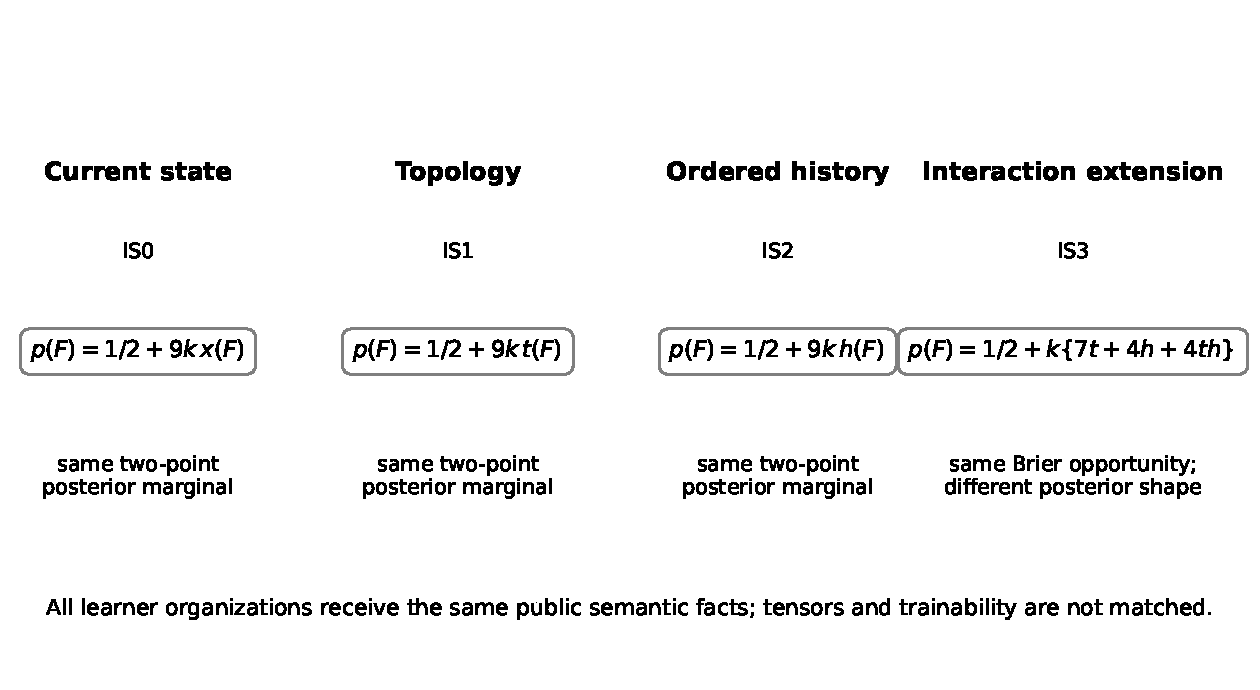
\includegraphics[width=0.98\linewidth]{figure1_design.pdf}
\caption{Design overview. In the three pure-relocation conditions, the same two-point posterior marginal is determined by current state, dependency topology, or ordered history (IS0--IS2) at each opportunity level. The separate topology--history interaction condition (IS3) matches Bayes Brier opportunity but has a different posterior shape. Every learner organization receives the same public semantic facts; the figure does not imply identical tensors or a required internal algorithm.}
\label{fig:design}
\end{figure}

All learner adapters preserve the same public semantic facts, including historical records. Static learners are not made history-blind, and temporal learners receive no privileged future information. This \textbf{semantic public-fact parity} controls information availability, not encoding geometry, bottlenecks, recurrent computation, effective capacity, numerical conditioning, or optimization. The current-state condition therefore also serves as an \textbf{implementation-gap control}: learner separation already present when topology and ordered history do not determine the posterior constrains how differences in the structurally dependent conditions can be interpreted.

The prospectively frozen primary estimands are six within-condition paired learner-system contrasts in size-integrated normalized regret (INR): Tabular versus Static for the topology-determined condition, Static versus Temporal for the ordered-history condition, and Static versus Temporal for the interaction extension, each at two opportunity levels. Patterns across conditions are development-stage descriptive comparisons rather than a confirmatory learner-by-regime interaction. Four specified learner--optimizer systems are evaluated under one frozen protocol using exact expected Brier risk over held-out public-support groups, which removes sampled evaluation-label noise while retaining training, corpus, initialization, and optimization variability.

The development comparison does not produce a uniform ranking. Mean size-integrated performance favors Temporal over Static at both ordered-history opportunity levels, while the topology and interaction contrasts change direction across opportunity levels. More importantly for interpretation, substantial Tabular--Static gaps are already present in the current-state control, where topology and ordered history do not determine the posterior. That observation prevents us from treating the primary contrasts as direct measures of relational or temporal reasoning and motivates a separate, explicitly post-hoc diagnostic layer on selected trajectories.

The diagnostic value is not the discovery of a new ReLU failure mode or a general learning-rate repair rule. Rather, the combination of a known posterior, exact expected-risk evaluation, shared public facts, exact trajectory replay, and interventions from the same pre-update state lets us distinguish two possibilities in selected cases: the information may be absent from the input, or it may remain present while a learned pathway loses the prediction-relevant distinction. The selected diagnostics do not explain the benchmark rankings as a whole; they show that this second failure mode can be isolated and probed directly.

The paper makes three contributions:
\begin{enumerate}
\item \textbf{Controlled information-location comparison.} We construct a finite-support benchmark in which three core conditions move an identical two-point posterior marginal among current state, topology, and ordered history, while a fourth interaction condition is explicitly separated as Brier-opportunity matched but not posterior-marginal matched.
\item \textbf{Finite-sample comparison with explicit estimands.} We evaluate specified tabular, static-graph, size-control, and graph-plus-GRU learner--optimizer systems with exact expected-risk evaluation and prospectively frozen within-condition contrasts. The matched core design removes posterior-marginal and Bayes-risk differences as explanations for descriptive cross-condition patterns while leaving representation and optimization differences visible.
\item \textbf{Selected diagnosis of learned-information retention.} Exact replay, bounded interventions, and frozen-state threshold analysis show, in selected trajectories, how prediction-relevant distinctions can be learned, lost, or retained without replacing the official benchmark results.
\end{enumerate}

The central message is not that one representation family wins. It is that \textbf{performance rankings alone are insufficient to diagnose relational or temporal information use, even when predictive opportunity and public information are tightly controlled}. Interpreting such comparisons requires separating how much predictive opportunity is present, which audited aspect of the public record determines the posterior, and whether a specified learning system can learn and stably retain the relevant distinction.

\section{Related Work}

Temporal graph learning provides many ways to organize evolving relational information. JODIE uses coupled recurrent embeddings; DyRep combines topology change and interaction dynamics; TGAT uses temporal attention; TGN combines event memory with graph operators; CAWN extracts anonymous temporal motifs; and PINT studies expressive temporal aggregation \citep{jodie,dyrep,tgat,tgn,cawn,pint}. Simpler alternatives such as GraphMixer, DyGFormer, and SimpleDyG, together with benchmarking efforts including TGB, TGB~2.0, and BenchTemp, broaden the comparison landscape \citep{graphmixer,dygformer,simpledyg,tgb,tgb2,benchtemp}. These works motivate the representation and evaluation setting, but our study does not propose a new temporal architecture, and the custom graph-plus-GRU learner is not intended as a reproduction of a named state-of-the-art system.

Controlled synthetic diagnosis is itself established methodology. GraphWorld varies parameterized graph-generating distributions and studies model rankings across sampled worlds; LRGB targets long-range dependencies under controlled model-size constraints; CLRS uses algorithmically generated trajectories and graph-oriented probes; TGB-Seq includes a synthetic sequential diagnostic; and ChaosNetBench varies controlled spatio-temporal dynamics \citep{graphworld,lrgb,clrs,tgbseq,chaosnet}. Our control is narrower: within IS0--IS2, the full posterior marginal is held fixed while the audited public statistic determining that posterior changes among current state, topology, and ordered history. This removes differences in posterior shape, prevalence, and Bayes-optimal Brier risk as explanations for descriptive differences across those regimes, while deliberately leaving representation and optimization difficulty uncontrolled.

The closest synthetic diagnostic comparison among the sources we examined is T-GRAB \citep{tgrab}. We inspected the final KDD 2026 paper. T-GRAB constructs separate synthetic tasks for periodicity, delayed cause-and-effect, and long-range spatial--temporal dependencies, comparing continuous-time, discrete-time, static, and heuristic methods primarily through link-prediction F1. Our pure-relocation conditions ask a different controlled question: IS0--IS2 keep the target-posterior marginal identical within an opportunity level while changing whether that posterior is determined by current state, topology, or ordered history in the shared public record. This removes posterior-marginal and Bayes-risk differences as explanations for descriptive cross-regime patterns in IS0--IS2, but not representation or trainability differences. Our evaluation is Bayes-referenced expected Brier risk, and an adapter audit establishes semantic public-fact parity across learner organizations. IS3 is analyzed separately because it matches Brier opportunity but not posterior shape. We state this as a methodological distinction, not a priority claim.

Other adjacent work further narrows the contribution boundary. A synthetic temporal-knowledge-graph distribution-shift study uses a generator-aware oracle, neural-prior stochastic block models provide explicit Bayes-referenced graph inference, and Grables formalizes table-to-graph construction and relational expressivity \citep{tkgshift,neuralprior,grables}. Known generators, Bayes references, and table--graph comparisons are therefore not novel ingredients by themselves. Likewise, inactive ReLUs, momentum-related death, oversquashing, and temporal-model degeneration under negative sampling have distinct prior literatures \citep{dyingrelu,momentumrelu,oversquashing,degeneration}. Our contribution is the particular controlled combination of shared public facts, posterior-marginal matching in IS0--IS2, exact Bayes-referenced risk evaluation, specified learner--optimizer comparisons, and bounded post-hoc diagnostics.

\section{Problem Formulation}

Let $F$ denote the complete normalized public record available at the prediction cutoff, $Y\in\{0,1\}$ the future binary target, and $p(F)=P(Y=1\mid F)$ the known synthetic posterior. A learner predicts $q(F)$. We use the binary one-component Brier convention
\[
B(q)=E[(Y-q(F))^2].
\]
This is half the two-component binary sum sometimes used in multicategory scoring; every baseline and normalization here uses the same convention. Quadratic probability evaluation follows \citet{brier}, within the proper-scoring framework of \citet{proper}.

For fixed $F$, expected loss is $p(1-q)^2+(1-p)q^2$. Consequently,
\[
B(q)=E[p(1-p)]+E[(q-p)^2].
\]
The Bayes risk is $B^*=E[p(1-p)]$, so excess Brier risk is the mean squared posterior-estimation error. With prevalence one half, the constant forecast has $B_0=1/4$. Predictive opportunity is
\[
\Delta=B_0-B^*=\operatorname{Var}(p).
\]
This identity permits exact opportunity matching without fitting an oracle learner. Matching the full marginal distribution of $p$ is stronger than matching only $\Delta$: IS0--IS2 satisfy the stronger control, whereas IS3 shares the same variance within an opportunity level but changes the posterior marginal.

We operationalize \textbf{information location} using three audited deterministic statistics of the same public record $F$. Let $x(F)\in\{-1,+1\}$ encode the latest low/high delivery warning, $t(F)\in\{-1,+1\}$ encode the public dependency topology (\texttt{join\_d} versus \texttt{merge\_c}), and $h(F)\in\{-1,+1\}$ encode the relative order of the two earlier low/high warnings. The signs are mathematical coordinates used by the generator and exact audit; regime identifiers, signs, and oracle posteriors are not learner input features. Each sign is nevertheless recoverable from the public records: $x$ from the current warning, $t$ from public dependency relations, and $h$ from timestamped warning history.

Thus ``location'' does not mean that one learner receives a fact that another learner does not. It identifies which audited public statistic determines the posterior under the frozen data-generating regime. This operational definition is deliberately narrower than a claim about minimal computational complexity, unique sufficient representations, or a causal architectural mechanism.

Normalized regret is $NR=(B-B^*)/\Delta$, and normalized recovery is $1-NR=(B_0-B)/\Delta$. We plot recovery multiplied by 100. It is not classification accuracy: zero corresponds to the constant baseline, 100 to the Bayes posterior, and negative values indicate worse risk than the baseline. Smaller $\Delta$ makes the same absolute excess risk appear larger after normalization; O1 and O2 must therefore be interpreted with their denominators visible.

\section{World Construction and Information-Location Control}

The frozen public support balances $x$, $t$, and $h$ independently, together with nuisance schedule contexts. For opportunity level $k$, the exact public posterior is
\begin{align}
p_{\mathrm{IS0}}(F)&=\tfrac12+9k\,x(F),\\
p_{\mathrm{IS1}}(F)&=\tfrac12+9k\,t(F),\\
p_{\mathrm{IS2}}(F)&=\tfrac12+9k\,h(F),
\end{align}
while
\[
p_{\mathrm{IS3}}(F)=\tfrac12+k\{7t(F)+4h(F)+4t(F)h(F)\}.
\]
O1 sets $k=1/128$; O2 sets $k=1/64$. These equations are not fitted summaries: exact enumeration of the frozen generator groups every public coordinate and verifies the displayed posterior formula.

For fixed $k$, IS0--IS2 share the same two-point posterior marginal $\{1/2-9k,1/2+9k\}$, each with probability $1/2$. We call these \textbf{pure relocation regimes} because the full posterior marginal is matched while the posterior-determining statistic changes from current state to topology to ordered history. Their prevalence, Bayes Brier opportunity, Bayes binary accuracy $E[\max(p,1-p)]$, and expected Bernoulli entropy $E[H_2(p)]$ are therefore identical. This control does not match encoding geometry, effective capacity, numerical conditioning, or optimization difficulty.

Orthogonality of the balanced signs gives $\operatorname{Var}(p)=81k^2$ for every regime within each opportunity level: $81/16384$ for O1 and $81/4096$ for O2. The corresponding Bayes risks are $4015/16384$ and $943/4096$. IS3 is an \textbf{interaction extension}, not a fourth posterior-shape-matched relocation condition. Its marginal places masses $1/2,1/4,1/4$ at $1/2-7k,1/2-k,1/2+15k$. It therefore shares prevalence and Brier opportunity with IS0--IS2 but not their Bayes binary accuracy or expected Bernoulli entropy. Exact enumeration verifies these statements over the full public support and within each frozen split.

In IS3, topology-only opportunity is $49k^2$, while the extra opportunity accessible with history given topology is $32k^2$. The product term contributes $16k^2$ under this orthogonal decomposition. These are properties of the imposed posterior and its Brier-risk decomposition; they are not identified real-world causal effects or a general partial-information-decomposition synergy measure.

The public support has 128 groups formed from the three core signs and nuisance schedule contexts. A frozen partition allocates 64 groups to training and 32 each to validation and test, preserving the complete core sign pattern within every split. Evaluation therefore concerns unseen combinations of familiar context factors, not unseen causal rules or unrestricted domain transfer. Large $N$ means more sampled training examples from this finite support, not thousands of distinct construction projects.

Every adapter preserves the same public semantic facts, including timestamps, earlier records, and typed references. Static is a non-recurrent organization of those records, not an input restricted to the latest state. Temporal adds derived sequence organization from the same public clocks and references. Tabular serializes the public records and reversible endpoint references into a learned MLP input. Adapter round-trip and invariance audits verify recoverability of the normalized public record. Oracle posteriors, regime identifiers, future labels, and hidden mathematical coordinates are excluded from learner inputs. Public-fact parity therefore prevents a privileged-information comparison, but it does not imply identical tensors, encoding geometry, effective capacity, numerical conditioning, or optimization behavior.

\begin{table}[t]
\centering
\caption{Information-location regimes and exact posterior controls. ``Marginal matched'' refers to the two-point posterior marginal shared by IS0--IS2 within an opportunity level.}
\label{tab:regimes}
\small
\begin{tabular}{lllll}
\toprule
Regime & Posterior driver & Posterior & Marginal matched & Brier opportunity \\
\midrule
IS0 & current state & $1/2+9kx$ & yes & matched \\
IS1 & topology & $1/2+9kt$ & yes & matched \\
IS2 & ordered history & $1/2+9kh$ & yes & matched \\
IS3 & topology/history & $1/2+k(7t+4h+4th)$ & no & matched \\
\bottomrule
\end{tabular}
\end{table}

\section{Learners and Frozen Training Protocol}

The four implementations contain 66,981 parameters for Tabular, 66,201 for Static, 69,085 for Static size control, and 70,377 for Temporal. Static uses two message-passing layers; Temporal combines graph processing with ordered GRU processing. The size control increases the static width. Tabular's content bottleneck has width 8, whereas the graph implementations use widths 24 or 25. Similar total counts therefore do not establish matched effective capacity.

\begin{table}[t]
\centering
\caption{Specified learner systems. Historical information is available to every system.}
\label{tab:learners}
\small
\begin{tabular}{lrlc}
\toprule
Family & Parameters & Organization & Content width \\
\midrule
Tabular & 66,981 & flattened records + endpoints + MLP & 8 \\
Static & 66,201 & two-layer message passing & 24 \\
Static size control & 69,085 & wider two-layer message passing & 25 \\
Temporal & 70,377 & message passing + ordered GRU & 24 \\
\bottomrule
\end{tabular}
\end{table}

All official runs use binary cross-entropy with logits, AdamW, initial learning rate 0.001, weight decay 0.0001, batch size 32, and 100 epochs. Final epoch 100 is the official endpoint; best diagnostic epochs never replace it. The implementations use float64 and deterministic execution. The protocol is frozen across conditions, so this is a comparison of specified learner--optimizer combinations, not independently optimized performance envelopes. AdamW follows the distinction between adaptive updates and decoupled weight decay described by \citet{adamw}.

Training sizes are 128, 512, 2,048, and 8,192. At a fixed epoch count, these sizes imply different update budgets: larger $N$ changes both data availability and the number of optimizer updates. A declining curve is therefore not by itself evidence that more data is harmful. The selected boundary analyses address this ambiguity locally, without identifying its population-wide contribution. Accordingly, these curves do not identify pure sample efficiency or sample complexity at a fixed update budget.

The run grid comprises eight regime/opportunity cells, four sizes, four families, six independently generated corpora, and three initialization replicates, totaling 2,304 runs. Initializations are nested replicates; the independent unit for the primary comparison is the corpus.

\section{Evaluation and Prospectively Frozen Analysis}

Each final model is evaluated by integrating Bernoulli labels analytically over the 32 held-out public groups. There is no sampled test-label noise in this expected-risk calculation. Training-label sampling, sampled training contexts, initialization, and optimization still vary. Exact evaluation should not be confused with certainty about a family-level effect.

For a fixed learner--optimizer system, regime, opportunity level, training size, corpus, and initialization, the observed quantity is exact held-out Brier risk and its Bayes-normalized regret. The primary size-integrated endpoint is
\[
INR=\frac{0.5\,NR_{128}+NR_{512}+NR_{2048}+0.5\,NR_{8192}}{3},
\]
the prospectively frozen trapezoidal weighting on equally spaced log-size levels. A contrast is $INR(\mathrm{left})-INR(\mathrm{right})$, so a positive value favors the right-hand learner. Paired differences are formed within each initialization and then averaged within a corpus; the six corpus values are the independent observations. A final-size recovery percentage is a different descriptive estimand and cannot substitute for INR.

The official primary estimands are six pre-specified paired learner-system contrasts, each evaluated separately at O1 and O2. C1 uses $INR(\mathrm{Tabular})-INR(\mathrm{Static})$ in IS1. C2 and C3 use $INR(\mathrm{Static})-INR(\mathrm{Temporal})$ in IS2 and IS3. Thus a positive value favors the right-hand learner in every primary contrast. IS0 learner contrasts are implementation-gap controls rather than additional primary superiority tests. Across-regime differences are secondary/descriptive; the study does not estimate a clean causal architecture effect or claim a statistically established regime-by-architecture interaction.

The measured contrasts belong to the specified learner--optimizer systems under the common frozen protocol. They should not be interpreted as isolated architecture effects: the IS0 implementation-gap control shows that representation, bottleneck, effective capacity, conditioning, and optimization can generate substantial separation even when topology and ordered history do not determine the posterior.

Stage V is development and variance-estimation evidence. Its six primary contrasts are displayed without confirmatory $p$-values, significance stars, or invented confidence intervals. The Stage C allocation reached $R=32$ but was not precision-feasible: the worst planned half-width was approximately 0.1553, above the 0.10 target. Stage C was not executed and no Stage C seeds were reserved. Reporting an allocation cap does not establish achieved precision.

Execution provenance includes a checkpoint migration, retained legacy runs, and prescribed replay checks. No performance-based exclusion or best-run selection was used.

\section{Development Results}

The development evidence is easiest to read in two layers before the post-hoc diagnostics. First, the primary INR contrasts integrate performance across all four training sizes, whereas a recovery value at $N=8{,}192$ is a single point on a learning curve and can therefore disagree with the size-integrated ranking. Second, the primary contrasts are mixed across conditions, and the IS0 implementation-gap control shows that those differences cannot be assigned to structural information use alone. Sections~\ref{sec:failure}--\ref{sec:interventions} then examine selected failure trajectories to ask how usable predictive distinctions can disappear during training; those diagnostics are not used to explain all official runs.

\begin{figure}[t]
\centering
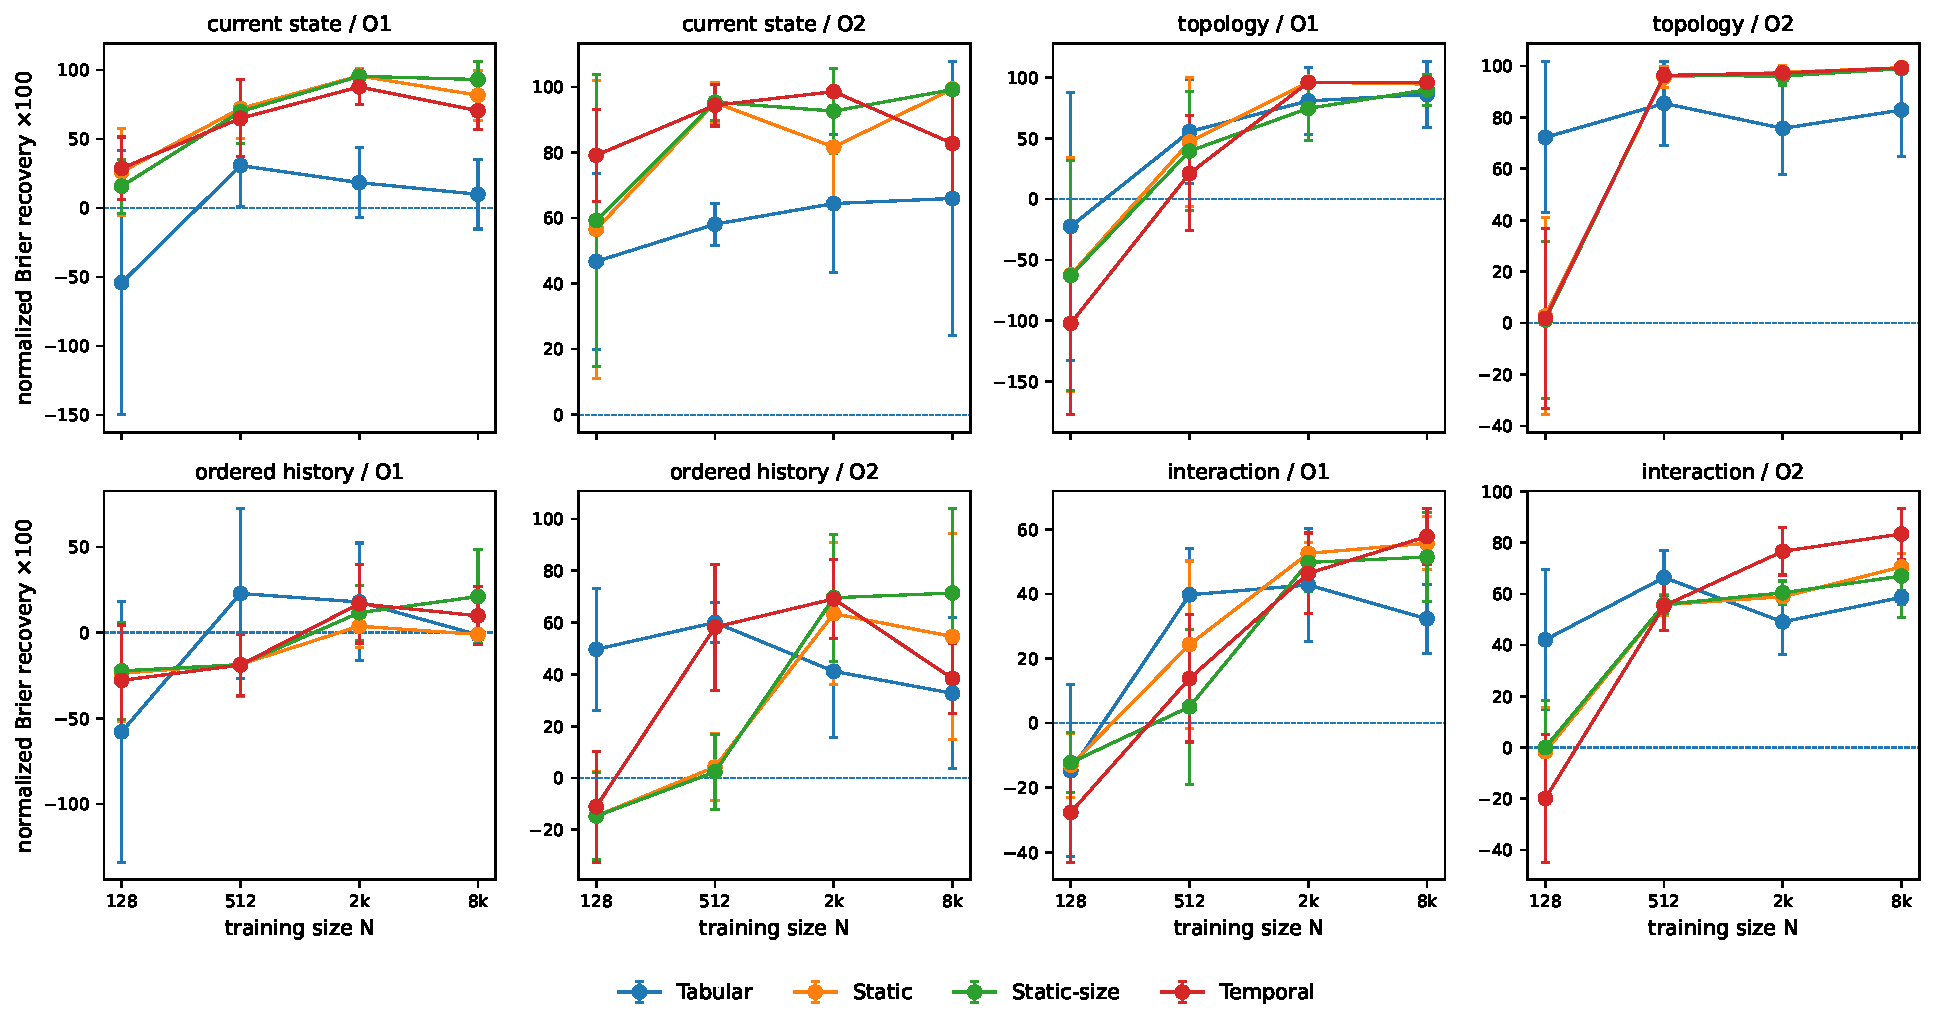
\includegraphics[width=\linewidth]{figure2_learning_curves.pdf}
\caption{Final-epoch normalized Brier recovery ($\times 100$; not accuracy) for the current-state control, topology-determined, ordered-history-determined, and interaction conditions, each at two opportunity levels. Lines and markers show means across six independent corpus means; error bars are corpus sample standard deviations and are descriptive, not confidence intervals. Higher is better.}
\label{fig:curves}
\end{figure}

\begin{table}[t]
\centering
\caption{Primary size-integrated INR contrasts. Positive differences favor the right-hand learner. Corpus sample SD is descriptive variability, not a confidence interval.}
\label{tab:primary}
\small
\begin{tabular}{llllrr}
\toprule
Contrast & Cell & Left & Right & Mean diff. & Corpus SD \\
\midrule
C1-O1 & IS1-O1 & Tabular & Static & -0.029065 & 0.213331 \\
C1-O2 & IS1-O2 & Tabular & Static &  0.018237 & 0.075669 \\
C2-O1 & IS2-O1 & Static & Temporal & 0.053517 & 0.060728 \\
C2-O2 & IS2-O2 & Static & Temporal & 0.177969 & 0.128925 \\
C3-O1 & IS3-O1 & Static & Temporal & -0.076447 & 0.058304 \\
C3-O2 & IS3-O2 & Static & Temporal & 0.048677 & 0.043438 \\
\bottomrule
\end{tabular}
\end{table}

\begin{figure}[t]
\centering
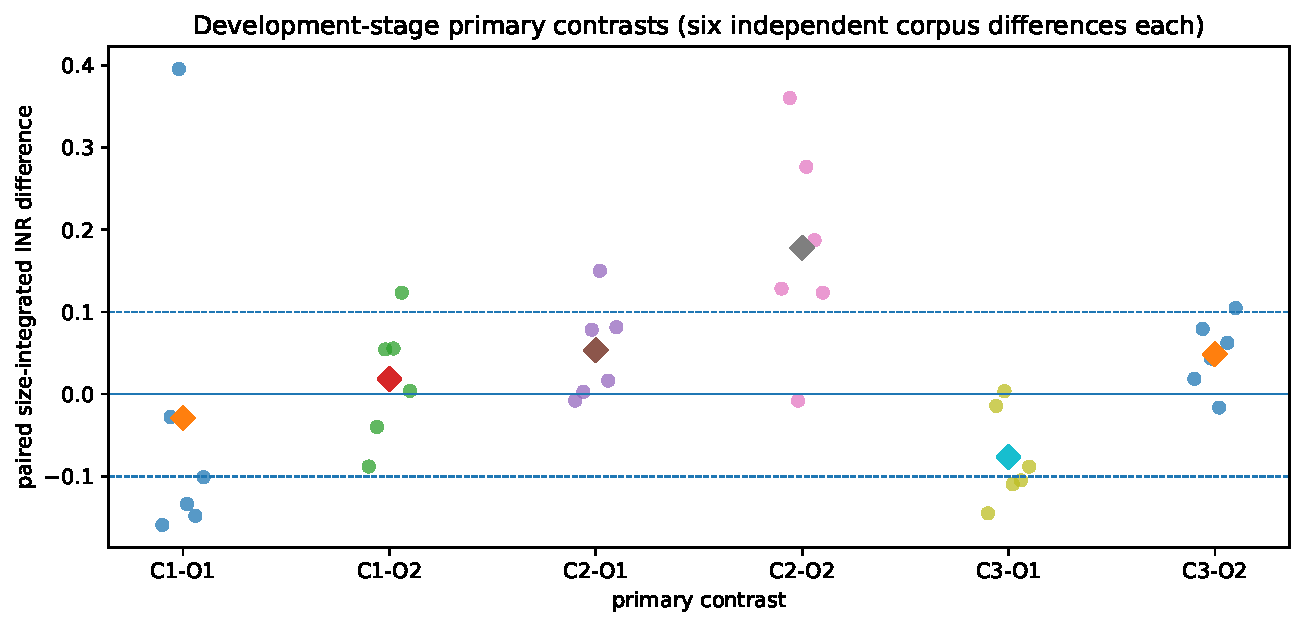
\includegraphics[width=0.92\linewidth]{figure3_primary_inr.pdf}
\caption{Six independent corpus differences per primary contrast and their mean. The plotted differences are left minus right: C1 is $INR(\mathrm{Tabular})-INR(\mathrm{Static})$, while C2 and C3 are $INR(\mathrm{Static})-INR(\mathrm{Temporal})$; positive values therefore favor the right-hand learner. Dashed $\pm0.10$ lines are a predeclared practical-margin reference only, not significance thresholds, confidence intervals, or achieved precision. These are development comparisons; the planned confirmatory stage was not run.}
\label{fig:inr}
\end{figure}

The primary system contrasts show no single ranking pattern. In the IS2 ordered-history-determined condition, $INR(\mathrm{Static})-INR(\mathrm{Temporal})$ is positive at both opportunity levels, so the mean C2 contrast favors Temporal. In IS1, $INR(\mathrm{Tabular})-INR(\mathrm{Static})$ changes sign between O1 and O2; in the IS3 interaction extension, $INR(\mathrm{Static})-INR(\mathrm{Temporal})$ also changes sign. These are development estimates within conditions, viewed descriptively across regimes; the experiment has not established a confirmatory learner-by-regime interaction.

The IS0 current-state implementation-gap control is the main constraint on interpreting those rankings. IS0 contains no posterior dependence on topology or ordered history, yet Tabular-minus-Static INR gaps are approximately 0.6489 at O1 and 0.2531 at O2. Thus, even when public information and predictive opportunity are controlled, learner separation can arise for reasons other than successful use of the regime's posterior-determining structural statistic. Representation, bottlenecks, effective capacity, numerical conditioning, and trainability remain possible contributors.

The distinction between INR and a final-size point is visible in IS2-O2. At $N=8{,}192$, Temporal's descriptive recovery is lower than Static's even though its size-integrated C2 INR contrast is positive. The two summaries answer different questions: INR averages normalized regret over the full size grid, whereas the $N=8{,}192$ recovery describes only the largest training size. This nonmonotonicity, together with the interpretive constraint exposed by IS0, motivated the selected diagnostic analyses that follow.

\section{Selected Failure Diagnostics}\label{sec:failure}

Cases were selected after inspecting official outcomes; they are not a representative sample from which to estimate failure prevalence. The diagnostic package includes both poor and good comparators. Instrumented replays matched prescribed final parameters, predictions, and metrics, establishing that the recorded failure trajectories correspond to the original runs rather than an instrumentation-induced substitute.

\begin{table}[t]
\centering
\caption{Selected diagnostic cases. Recovery is normalized Brier recovery $\times100$, not classification accuracy.}
\label{tab:cases}
\small
\begin{tabular}{llllrr}
\toprule
Case & Family & Role & Cell / size & Final recovery & Death step \\
\midrule
D1 & Tabular & selected poor & IS2-O1 / 8192 & -0.995764 & 12,417 \\
D2 & Tabular & good comparator & IS2-O1 / 2048 & 94.849408 & -- \\
D3 & Temporal & selected poor & IS2-O1 / 8192 & -0.000607 & 2,742 \\
D4 & Temporal & good comparator & IS2-O1 / 8192 & 98.445644 & -- \\
\bottomrule
\end{tabular}
\end{table}

D1 and D3 lose all positive content activations at updates 12,417 and 2,742 respectively; D2 and D4 do not exhibit that event in their traced runs. Here content death means that the post-ReLU content representation is zero across the inspected public support. Paired inputs differing in the historical signal then lose their content-path distinction. This does not imply that every parameter, graph edge, bias, or downstream state is zero. Other graph pathways can retain topological distinctions. The mechanistic claim is restricted to the measured pathway and the selected task.

\begin{figure}[t]
\centering
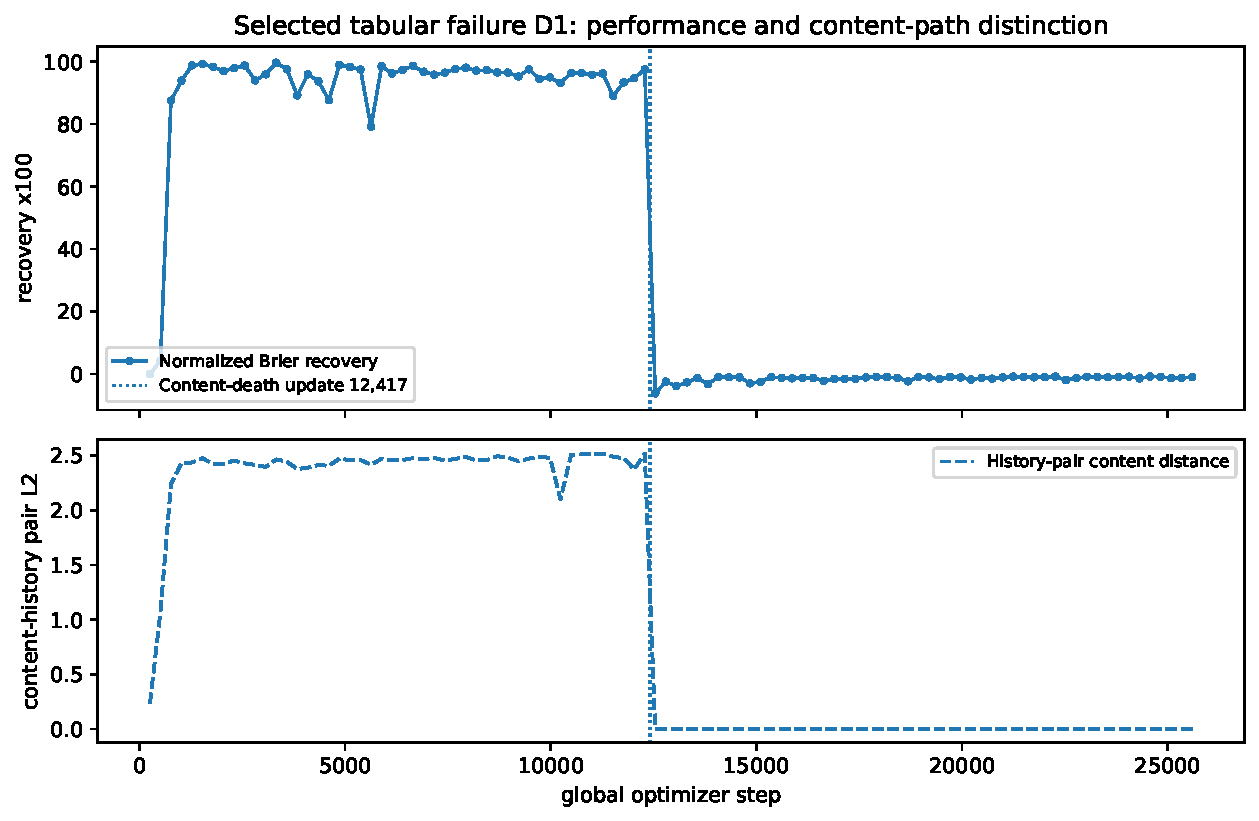
\includegraphics[width=0.92\linewidth]{figure4_d1_trajectory.pdf}
\caption{Global-step-aligned trajectory for the selected tabular failure D1, shown as two aligned panels to distinguish the quantities. The upper panel is epoch-end normalized Brier recovery; the lower panel is the measured history-pair content distance. The vertical dotted line marks the exact content-death update 12,417. The run reached 99.6659\% recovery at epoch 13 but had already fallen to 3.5031\% immediately before the boundary. The boundary is not the onset of all deterioration.}
\label{fig:d1}
\end{figure}

Frozen optimizer counterfactuals reconstructed the update on copies of the same prestate. For D1 and D3, removing immediate decay did not prevent death; retaining prior moments with zero current gradient and retaining current gradient with zero prior moments each still caused death in the specified artificial update. Suppressing the content update preserved its activity.

\begin{table}[t]
\centering
\caption{Frozen one-step optimizer counterfactuals. ``Dead'' means the inspected post-ReLU content pathway is all zero after the artificial update.}
\label{tab:counterfactuals}
\small
\begin{tabular}{lllr}
\toprule
Case & Counterfactual & Dead & Max preactivation \\
\midrule
D1 & original & yes & -0.055778 \\
D1 & no immediate decay & yes & -0.055778 \\
D1 & zero current gradient; retain prior moments & yes & -0.037904 \\
D1 & zero prior moments; retain current gradient & yes & -0.055778 \\
D1 & no content update & no & 0.051905 \\
D3 & original & yes & -0.012532 \\
D3 & no immediate decay & yes & -0.012532 \\
D3 & zero current gradient; retain prior moments & yes & -0.012532 \\
D3 & zero prior moments; retain current gradient & yes & -0.012532 \\
D3 & no content update & no & 0.000599 \\
\bottomrule
\end{tabular}
\end{table}

These tests show local sufficiency under artificial interventions, not a unique root cause. Resetting moments changes the adaptive denominator as well as history, so the variants cannot be summed into additive causal percentages. Immediate decay was neither necessary for the observed death nor sufficient in the decay-only check. Historical regularization or earlier gradient dynamics remain possible contributors to reaching the boundary.

\section{Selected Optimizer Interventions and Local Boundaries}\label{sec:interventions}

Starting from D1's exact pre-boundary state after 12,416 updates, a persistent reduction from 0.001 to 0.0001 at update 12,417 prevented complete content-path loss and subsequently recovered to 97.0827\% final normalized Brier recovery. Performance immediately before intervention was only 3.5031\%; the intervention did not maintain an uninterrupted high-performance state. The official D1 endpoint remains $-0.995764\%$. A separate intervention applied 0.0001 for only that one update and restored 0.001 for the next; it died at update 12,418 and ended at $-0.994286\%$. Immediate one-step survival therefore did not suffice for sustained recovery in this selected trajectory.

D3 received the persistent nominal reduction at its own boundary update 2,742. Content still died at that update; final recovery was $-0.000521796\%$, compared with the official $-0.000606841\%$. This result did not create a surviving content path and then test whether downstream temporal processing could recover. It cannot support the claim that Temporal is inherently less recoverable than Tabular.

\begin{figure}[t]
\centering
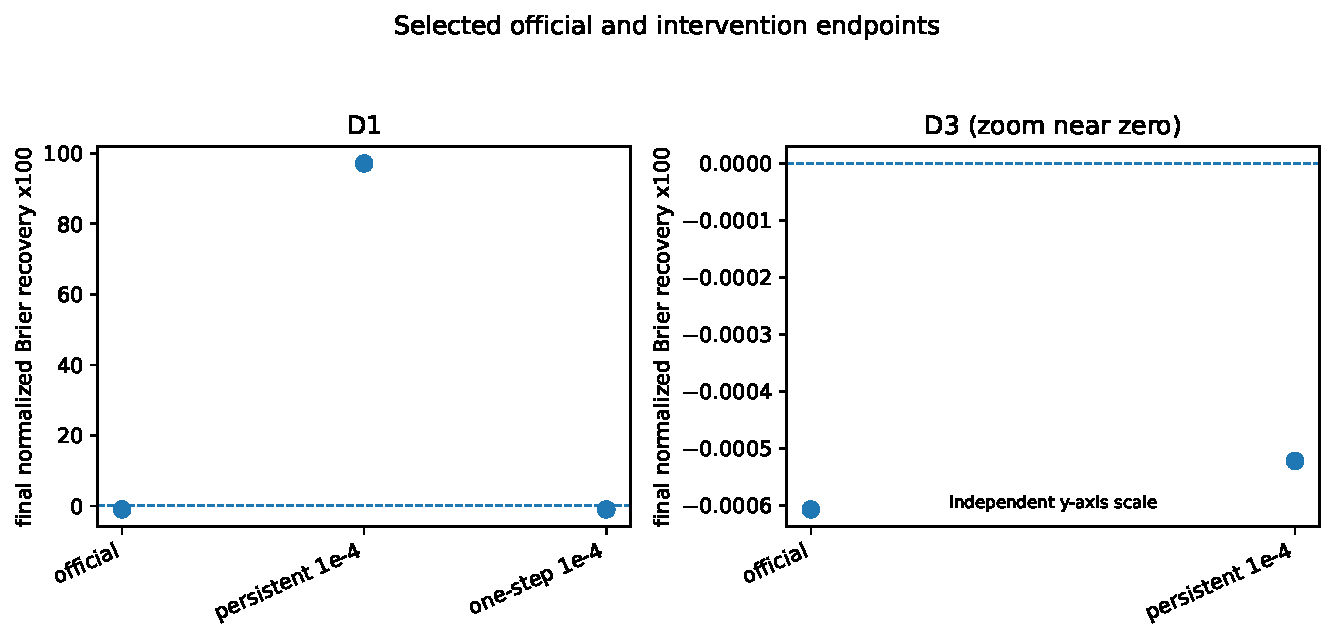
\includegraphics[width=0.82\linewidth]{figure5_interventions.pdf}
\caption{Final normalized Brier recovery for selected official and intervention continuations. The D1 and D3 panels use independent vertical scales; vertical distances must not be compared across panels, and D3 is a near-zero zoom. D1 persistent low learning rate prevents content death and ends with high recovery; the one-step D1 intervention and the persistent D3 intervention do not. Normalized Brier recovery is not classification accuracy. These are selected continuations, not randomized family-level arms, and they do not replace the official benchmark endpoints.}
\label{fig:interventions}
\end{figure}

For each exact frozen prestate and gradient, the one-step AdamW content update is affine in learning rate, up to floating-point evaluation. A content preactivation can therefore be expressed as $z_j(\eta)=a_j+\eta b_j$. The dead predicate requires every inspected activation to be nonpositive. Its transition is determined by an intersection of activation constraints; the maximum activation need not be globally monotone for arbitrary states.

The numerical alive/dead brackets were $[0.00046262514200061573, 0.0004626251426626627]$ for D1 and $[0.000032064047577380244, 0.00003206404820084572]$ for D3. Midpoints are numerical summaries, not exact mathematical roots. Dividing the applied 0.0001 by these midpoints gives approximately 0.21616 for D1 and 3.11876 for D3. Thus the same nominal tenfold reduction lies below D1's immediate-death boundary and above D3's.

\begin{figure}[t]
\centering
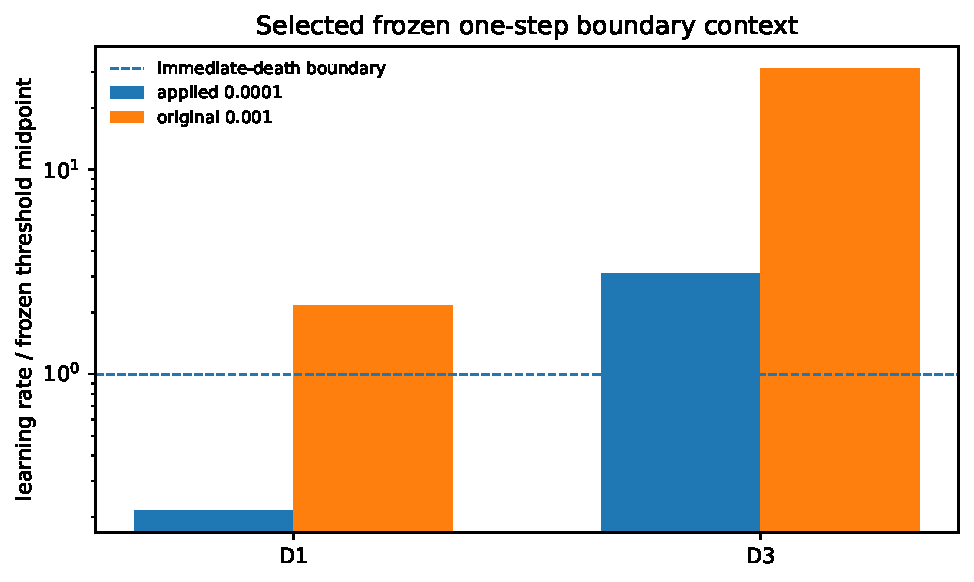
\includegraphics[width=0.72\linewidth]{figure6_boundary_normalized_lr.pdf}
\caption{Applied learning rate divided by the frozen one-step threshold midpoint. A value of 1 marks the selected state's immediate-death transition. The normalization describes a single update; it neither recommends an optimal learning rate nor predicts multi-step success.}
\label{fig:boundary}
\end{figure}

These probes support a local sequence of claims: D1's sustained schedule changed the selected outcome; a one-step schedule did not sustain it; D3's nominally identical schedule did not produce equivalent immediate survival. The probes do not isolate model family, initialization, boundary geometry, or content width as a population-level cause.

\section{Discussion}

The experiment yields a positive finding and a corresponding interpretive limit at each evidence level. At the design level, IS0--IS2 show that the same posterior marginal and the same public semantic facts can be paired with different posterior-determining statistics; therefore, posterior shape and Bayes Brier opportunity need not change when the location of the predictive statistic changes. At the learner-system level, the observed rankings are condition dependent rather than uniform; however, the large IS0 implementation gaps show that those rankings cannot be attributed to architecture or structural-information use alone. At the mechanistic level, selected replays demonstrate that a learned content pathway can lose the distinction needed for prediction while the source information remains present in the inputs; however, those selected cases do not establish how often that mechanism occurs or whether it explains the full benchmark.

\subsection{Semantic parity and learner-system interpretation}

Semantic public-fact parity controls what information is available, not how easily each learner can encode, propagate, or optimize it. A graph model should not win simply because another learner was denied historical records or topology facts, but equal semantic access does not imply equal tensors, bottlenecks, recurrent computation, effective capacity, conditioning, or optimizer sensitivity. The large IS0 gaps make this concrete: substantial learner separation occurs even when topology and ordered history do not determine the posterior.

This distinction changes how the primary results should be read. The positive $INR(\mathrm{Static})-INR(\mathrm{Temporal})$ mean in both IS2 opportunity levels is evidence about the specified systems under the frozen protocol, not a direct measurement of an abstract temporal-reasoning capability. Likewise, the sign changes in IS1 and IS3 do not show that topology or temporal structure is uninformative. The benchmark therefore narrows one ambiguity---posterior difficulty in IS0--IS2---without eliminating representation and optimization as competing explanations.

The selected interventions add a second useful distinction. In D1, a persistent learning-rate reduction from the exact pre-boundary state prevented complete content-path loss and was followed by high final recovery, whereas a one-step reduction delayed death by only one update and did not recover performance. In D3, the same nominal persistent reduction did not prevent immediate content death because it remained above that selected state's frozen one-step boundary. These results establish local state-dependent optimization behavior, not a general optimal learning rate or a family-wide difference in recoverability.

\subsection{Implications}

The controlled benchmark suggests a practical diagnostic sequence for future empirical work. First ask what predictive opportunity is available. Then ask which observable current facts, dependency relations, or ordered histories determine the target risk. Finally ask whether the chosen learning system can learn and stably retain the relevant distinction under realistic data and compute constraints. This ordering helps separate missing information, representation difficulty, and optimization failure before assigning a result to relational or temporal reasoning.

Fixed epochs remain an important qualification: increasing training size also increases optimizer-update count, so the curves do not identify pure sample complexity at a fixed compute budget. The construction vocabulary is also only an interpretable synthetic setting; the present results do not establish predictive accuracy, workflow improvement, cost reduction, or business value in real construction settings. Replicating the mechanism findings at a broader level would require independently selected trajectories, a pre-specified selection rule, and fixed diagnostic endpoints; no such replication was performed here.

\section{Limitations}

The world is deliberately small, finite, and analytically designed. It does not capture construction-domain interventions, missingness, unobserved confounding, organizational behavior, or open-ended graph size. Context-disjoint splits preserve the core signal patterns rather than testing new causal rules. Across all four regimes, the common opportunity control concerns Brier risk and prevalence; only IS0--IS2 also match the full posterior marginal, posterior-only Bayes accuracy, and entropy. IS3 therefore cannot be pooled with the pure-relocation regimes as an information-location-only comparison.

The learner set is narrow and custom. There is no tree-ensemble baseline, broad hyperparameter search, or direct replication of TGN, DyGFormer, or other named literature architectures. Parameter-count proximity does not equalize effective capacity or compute, and fixed epochs couple training size to optimizer-update count. The results describe the frozen learner--optimizer systems rather than optimized performance envelopes for representation families.

Stage V contains six independent corpora and is development-only. The prospective Stage C precision gate was not feasible within the selected allocation cap, so no confirmatory Stage C comparison was executed. Repeated inspection and post-hoc case selection further limit mechanistic inference: the selected content-path failures cannot be assigned a population prevalence or used to explain all official results.

The optimizer interventions are local to particular prestates, gradients, and schedules. They alter the optimizer schedule for all parameter groups, and the frozen one-step thresholds do not identify generally safe or optimal learning rates. D1 and D3 also differ in architecture, initialization, and training state, so their boundary differences are not a controlled model-family comparison.

Finally, the literature review is scoped rather than exhaustive. The final KDD 2026 T-GRAB paper was inspected for the methodological comparison used here, but the broader literature search is not a field-wide proof of priority. This paper therefore makes no first/only claim and states its contribution positively through the experimental design.

\section{Conclusion}

We operationalized \textbf{information location} as which audited statistic of a shared public record determines a synthetic target posterior. In the three core conditions, current state, topology, and ordered history determine the same two-point posterior marginal within each opportunity level; the separate topology--history interaction extension matches Bayes Brier opportunity but not posterior shape.

The development experiment produced three concrete observations. First, learner-system rankings were not uniform: mean size-integrated normalized regret favored Temporal over Static at both ordered-history opportunity levels, while the topology and interaction contrasts changed sign across opportunity levels. Second, substantial Tabular--Static gaps also appeared in the current-state control, where topology and ordered history do not determine the posterior. That result shows why rankings under structural conditions cannot be interpreted as isolated measures of relational or temporal information use. Third, selected post-hoc trajectories showed that a learned content pathway can lose a prediction-relevant distinction even while the underlying public information remains available. In one selected tabular failure, a persistent learning-rate reduction from the exact pre-boundary state prevented complete content-path loss and was followed by 97.0827\% final normalized Brier recovery; a one-step reduction was insufficient. In a selected temporal failure, the same nominal persistent reduction did not prevent immediate content death.

Together, these results support a diagnostic view of representation comparisons: \textbf{predictive opportunity, the public statistic that determines the posterior, and the ability of a learning system to learn and stably retain the relevant distinction are separate empirical questions}. The evidence remains development-stage---the planned confirmatory stage was not executed, the learner set is narrow, and the mechanism cases are selected---so it does not establish a universal model ranking, a causal architecture effect, a general repair method, or construction-domain performance.

\section{Reproducibility Notes}

A publication-clean reproducibility repository is available at \url{https://github.com/k3ijo-miyamoto/information-location-benchmark}. The version referenced by this preprint is commit \texttt{b38f6f1aa8f5486b99427b3e7af4741f1a7270d9}. It contains the Generator 1.3 design, learner/evaluator implementation, frozen public configurations, exact design audits, Stage V aggregate analysis, the Stage C allocation record, selected diagnostic summaries, and CPU-friendly scripts that verify the paper-level numerical claims and regenerate publication tables/figures from committed evidence. The full 2,304-run training rerun is not required for this paper-level verification and is not claimed to be bitwise portable across arbitrary hardware. The audit trail is separate from the scientific evidence: it checks correspondence among public artifacts and reported quantities but does not upgrade development evidence to confirmation.

\begin{thebibliography}{99}

\bibitem[Kumar et~al.(2019)Kumar, Zhang, and Leskovec]{jodie}
Srijan Kumar, Xikun Zhang, and Jure Leskovec.
\newblock Predicting dynamic embedding trajectory in temporal interaction networks.
\newblock In \emph{Proceedings of the 25th ACM SIGKDD International Conference on Knowledge Discovery \& Data Mining}, 2019.
\newblock doi:10.1145/3292500.3330895.

\bibitem[Trivedi et~al.(2019)Trivedi, Farajtabar, Biswal, and Zha]{dyrep}
Rakshit Trivedi, Mehrdad Farajtabar, Prasenjeet Biswal, and Hongyuan Zha.
\newblock DyRep: Learning representations over dynamic graphs.
\newblock In \emph{International Conference on Learning Representations}, 2019.

\bibitem[Xu et~al.(2020)Xu, Ruan, Korpeoglu, Kumar, and Achan]{tgat}
Da Xu, Chuanwei Ruan, Evren Korpeoglu, Sushant Kumar, and Kannan Achan.
\newblock Inductive representation learning on temporal graphs.
\newblock In \emph{International Conference on Learning Representations}, 2020.

\bibitem[Rossi et~al.(2020)Rossi, Chamberlain, Frasca, Eynard, Monti, and Bronstein]{tgn}
Emanuele Rossi, Ben Chamberlain, Fabrizio Frasca, Davide Eynard, Federico Monti, and Michael Bronstein.
\newblock Temporal graph networks for deep learning on dynamic graphs.
\newblock \emph{arXiv preprint arXiv:2006.10637}, 2020.

\bibitem[Wang et~al.(2021)Wang, Chang, Liu, Leskovec, and Li]{cawn}
Yanbang Wang, Yen-Yu Chang, Yunyu Liu, Jure Leskovec, and Pan Li.
\newblock Inductive representation learning in temporal networks via causal anonymous walks.
\newblock In \emph{International Conference on Learning Representations}, 2021.

\bibitem[Souza et~al.(2022)Souza, Mesquita, Kaski, and Garg]{pint}
Amauri H. Souza, Diego Mesquita, Samuel Kaski, and Vikas Garg.
\newblock Provably expressive temporal graph networks.
\newblock In \emph{Advances in Neural Information Processing Systems}, 2022.

\bibitem[Cong et~al.(2023)Cong et~al.]{graphmixer}
Weilin Cong et~al.
\newblock Do we really need complicated model architectures for temporal networks?
\newblock In \emph{International Conference on Learning Representations}, 2023.

\bibitem[Yu et~al.(2023)Yu, Sun, Du, and Lv]{dygformer}
Le Yu, Leilei Sun, Bowen Du, and Weifeng Lv.
\newblock Towards better dynamic graph learning: New architecture and unified library.
\newblock In \emph{Advances in Neural Information Processing Systems}, 2023.

\bibitem[Wu et~al.(2024)Wu, Fang, and Liao]{simpledyg}
Yuxia Wu, Yuan Fang, and Lizi Liao.
\newblock On the feasibility of simple transformer for dynamic graph modeling.
\newblock In \emph{Proceedings of the ACM Web Conference}, 2024.
\newblock doi:10.1145/3589334.3645622.

\bibitem[Huang et~al.(2023)Huang et~al.]{tgb}
Shenyang Huang et~al.
\newblock Temporal graph benchmark for machine learning on temporal graphs.
\newblock In \emph{Advances in Neural Information Processing Systems, Datasets and Benchmarks Track}, 2023.

\bibitem[Gastinger et~al.(2024)Gastinger et~al.]{tgb2}
Julia Gastinger, Shenyang Huang, Mikhail Galkin, Erfan Loghmani, Ali Parviz, Farimah Poursafaei, Jacob Danovitch, Emanuele Rossi, Ioannis Koutis, Heiner Stuckenschmidt, Reihaneh Rabbany, and Guillaume Rabusseau.
\newblock TGB 2.0: A benchmark for learning on temporal knowledge graphs and heterogeneous graphs.
\newblock In \emph{Advances in Neural Information Processing Systems, Datasets and Benchmarks Track}, 2024.

\bibitem[Huang et~al.(2024)Huang et~al.]{benchtemp}
Qiang Huang, Xin Wang, Susie Xi Rao, Zhichao Han, Zitao Zhang, Yongjun He, Quanqing Xu, Yang Zhao, Zhigao Zheng, and Jiawei Jiang.
\newblock BenchTemp: A general benchmark for evaluating temporal graph neural networks.
\newblock In \emph{IEEE International Conference on Data Engineering}, 2024.
\newblock doi:10.1109/ICDE60146.2024.00310.

\bibitem[Yi et~al.(2025)Yi et~al.]{tgbseq}
Lu Yi, Jie Peng, Yanping Zheng, Fengran Mo, Zhewei Wei, Yuhang Ye, Zixuan Yue, and Zengfeng Huang.
\newblock TGB-Seq Benchmark: Challenging temporal GNNs with complex sequential dynamics.
\newblock In \emph{International Conference on Learning Representations}, 2025.

\bibitem[Dizaji et~al.(2026)Dizaji et~al.]{tgrab}
Alireza Dizaji, Benedict Aaron Tjandra, Mehrab Hamidi, Shenyang Huang, and Guillaume Rabusseau.
\newblock T-GRAB: A synthetic diagnostic benchmark for learning on temporal graphs.
\newblock In \emph{Proceedings of the 32nd ACM SIGKDD Conference on Knowledge Discovery and Data Mining}, pages 2628--2639, 2026.
\newblock doi:10.1145/3770854.3785699.

\bibitem[Palowitch et~al.(2022)Palowitch, Tsitsulin, Mayer, and Perozzi]{graphworld}
John Palowitch, Anton Tsitsulin, Brandon Mayer, and Bryan Perozzi.
\newblock GraphWorld: Fake graphs bring real insights for GNNs.
\newblock In \emph{Proceedings of the 28th ACM SIGKDD Conference on Knowledge Discovery and Data Mining}, 2022.
\newblock doi:10.1145/3534678.3539203.

\bibitem[Dwivedi et~al.(2022)Dwivedi et~al.]{lrgb}
Vijay Prakash Dwivedi, Ladislav Rampasek, Michael Galkin, Ali Parviz, Guy Wolf, Anh Tuan Luu, and Dominique Beaini.
\newblock Long Range Graph Benchmark.
\newblock In \emph{Advances in Neural Information Processing Systems}, 2022.

\bibitem[Velickovic et~al.(2022)Velickovic et~al.]{clrs}
Petar Velickovic, Adria Puigdomenech Badia, David Budden, Razvan Pascanu, Andrea Banino, Misha Dashevskiy, Raia Hadsell, and Charles Blundell.
\newblock The CLRS algorithmic reasoning benchmark.
\newblock In \emph{Proceedings of the 39th International Conference on Machine Learning}, volume 162 of \emph{Proceedings of Machine Learning Research}, 2022.

\bibitem[Moges et~al.(2026)Moges, Skokos, and Moodley]{chaosnet}
Henok Tenaw Moges, Charalampos Skokos, and Deshendran Moodley.
\newblock ChaosNetBench: Benchmarking spatio-temporal graph neural networks on chaotic lattice dynamics.
\newblock \emph{arXiv preprint arXiv:2605.09676}, 2026.

\bibitem[Ozdemir et~al.(2026)Ozdemir et~al.]{tkgshift}
Konrad Ozdemir, Julia Gastinger, Lukas Kirchdorfer, and Heiner Stuckenschmidt.
\newblock Temporal knowledge graph forecasting under distribution shifts: A synthetic evaluation.
\newblock \emph{arXiv preprint arXiv:2607.09232}, 2026.

\bibitem[Duranthon and Zdeborova(2023)]{neuralprior}
O. Duranthon and L. Zdeborova.
\newblock Neural-prior stochastic block model.
\newblock \emph{Machine Learning: Science and Technology}, 4:035017, 2023.
\newblock doi:10.1088/2632-2153/ace60f.

\bibitem[Cucumides and Geerts(2026)]{grables}
Tamara Cucumides and Floris Geerts.
\newblock Grables: Tabular learning beyond independent rows.
\newblock \emph{arXiv preprint arXiv:2602.03945}, 2026.

\bibitem[Lu et~al.(2020)Lu, Shin, Su, and Karniadakis]{dyingrelu}
Lu Lu, Yeonjong Shin, Yanhui Su, and George Em Karniadakis.
\newblock Dying ReLU and initialization: Theory and numerical examples.
\newblock \emph{Communications in Computational Physics}, 2020.
\newblock doi:10.4208/cicp.OA-2020-0165.

\bibitem[Arnekvist et~al.(2020)Arnekvist et~al.]{momentumrelu}
Isac Arnekvist, J. Frederico Carvalho, Danica Kragic, and Johannes A. Stork.
\newblock The effect of target normalization and momentum on dying ReLU.
\newblock \emph{arXiv preprint arXiv:2005.06195}, 2020.

\bibitem[Alon and Yahav(2021)]{oversquashing}
Uri Alon and Eran Yahav.
\newblock On the bottleneck of graph neural networks and its practical implications.
\newblock In \emph{International Conference on Learning Representations}, 2021.

\bibitem[Daniluk and Dabrowski(2023)]{degeneration}
Michal Daniluk and Jacek Dabrowski.
\newblock Temporal graph models fail to capture global temporal dynamics.
\newblock \emph{arXiv preprint arXiv:2309.15730}, 2023.

\bibitem[Gneiting and Raftery(2007)]{proper}
Tilmann Gneiting and Adrian E. Raftery.
\newblock Strictly proper scoring rules, prediction, and estimation.
\newblock \emph{Journal of the American Statistical Association}, 102(477):359--378, 2007.
\newblock doi:10.1198/016214506000001437.

\bibitem[Brier(1950)]{brier}
Glenn W. Brier.
\newblock Verification of forecasts expressed in terms of probability.
\newblock \emph{Monthly Weather Review}, 78(1):1--3, 1950.

\bibitem[Loshchilov and Hutter(2019)]{adamw}
Ilya Loshchilov and Frank Hutter.
\newblock Decoupled weight decay regularization.
\newblock In \emph{International Conference on Learning Representations}, 2019.

\end{thebibliography}


\end{document}
